\section*{Results}

\begin{table}[htbp]


\begin{tabular}{lllll}
\toprule
{} & samples (RNA) &         Mutatisourons &   Neoantigens & Expressed Neoantigens \\
\midrule
ascites pre-treatment                 &         4 (4) &   10336 $\pm$ 800 &  202 $\pm$ 60 &           78 $\pm$ 30 \\
ascites post-treatment                &       24 (20) &  13757 $\pm$ 1000 &  300 $\pm$ 50 &          145 $\pm$ 30 \\
\textit{model adjusted change (\%)} &               &       55 $\pm$ 64 &  67 $\pm$ 100 &         128 $\pm$ 152 \\
\hline
solid pre-treatment                   &       75 (69) &    7902 $\pm$ 900 &  155 $\pm$ 20 &            65 $\pm$ 9 \\
solid post-treatment                  &        12 (5) &  11250 $\pm$ 3000 &  253 $\pm$ 80 &           38 $\pm$ 20 \\
\textit{model adjusted change (\%)}   &               &        7 $\pm$ 27 &    5 $\pm$ 38 &          -41 $\pm$ 32 \\
\bottomrule
\end{tabular}



\caption{\textbf{Mean mutations, neoantigens, and expressed noeantigens by sample type and chemotherapy treatment status.} The model-adjusted change is calculated using a Bayesian model that controls for technical variables affecting mutation identification, but does not separate treatment from coincident effects such as surgery and drift. Model effects and means are shown with 95\% credible regions and bootstrap errors of the mean, respectively.}
\label{tab:cohort}
\end{table}

\begin{figure}[htbp]
\centering
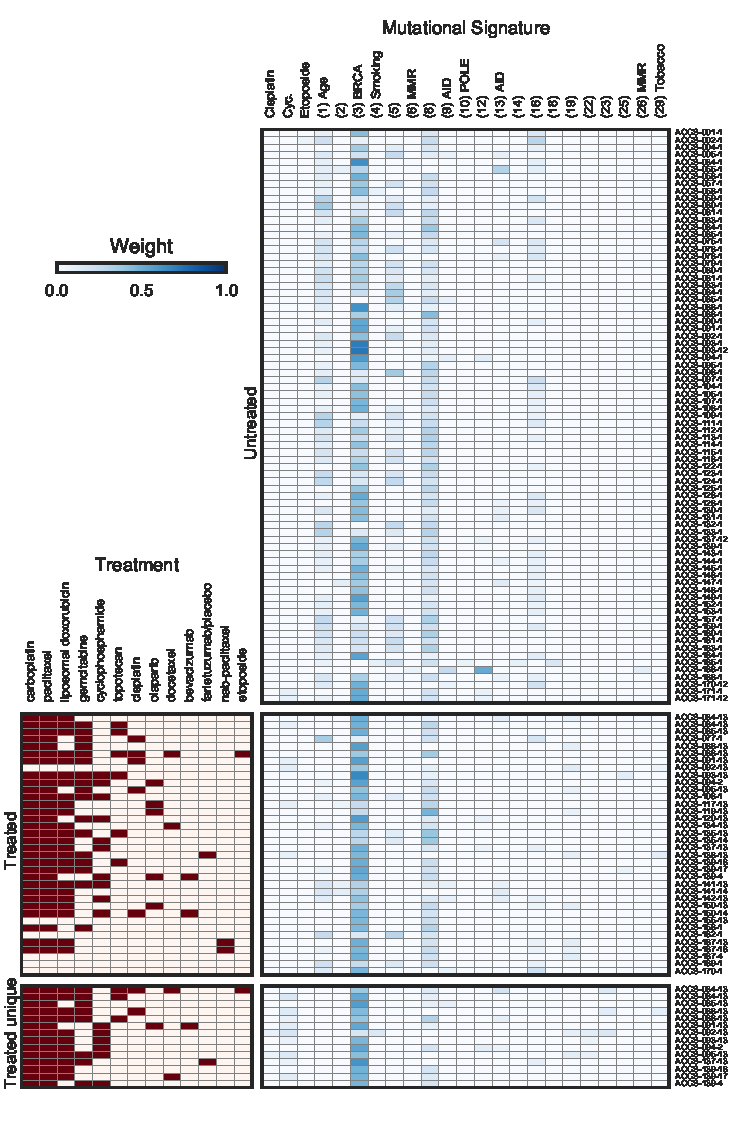
\includegraphics[scale=1.0]{figures/signatures.pdf}
\caption{\textbf{Treatments and mutational signature deconvolutions for paired pre-/post-chemotherapy samples.} \textit{(Top)} Signature deconvolution of the pre-treatment samples. The first five signatures were extracted from reports of a \textit{G. gallus}\cite{Szikriszt_2016} cell line and \textit{C. Elegans}\cite{Meier_2014} organisms after exposure to chemotherapy. The remaining signatures are from the COSMIC signature resource\cite{364242} and give the COSMIC signature number in parenthesis. Signatures not shown received no attribution across these samples. \textit{(Bottom)} Clinical treatments and signature deconvolutions for the mutations detectable only in post-treatment samples. Each case where a chemotherapy signature is detected is annotated with its level of agreement with the clinical record. A (*) indicates the donor received the drug, a (+) indicates the donor received a drug in the same family (platinum compounds), and a (?) indicates no record of the donor receiving a similar drug.}
\label{fig:signatures}
\end{figure}

\begin{figure}[htbp]
\centering
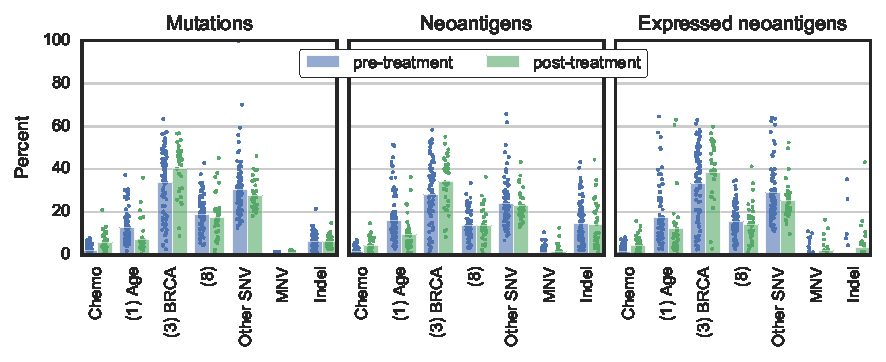
\includegraphics[scale=1.0]{figures/sources_of_mutations_and_neoantigens.pdf}
\caption{\textbf{Sources of mutations and neoantigens.}  The mean fraction of mutations \textit{(left)} and neoantigens \textit{(right)} generated by each signature across samples is plotted. SNVs are grouped by signature: ``chemo'' combines the signatures extracted from the \textit{G. gallus} and \textit{C. Elegans} studies, COSMIC signature numbers are in parentheses, the ``other'' category shows SNVs from COSMIC signatures other than the ones shown, and the ``unclassified'' category shows SNVs that were not accounted for by the signature deconvolution (unknown signatures or a mix of many processes). Multinucleotide variants (MNVs) and indels, which are not included in the signature deconvolution, are shown separately. Error bars show the 95\% error of the mean by bootstrapping on samples.}
\label{fig:sources}
\end{figure}
% The number of SNVs and neoantigens generated by each signature was estimated by summing over the mutations or neoantigens in a sample the posterior probability that the signature generated the mutation.

\subsection*{Change in mutations and neoantigens at recurrence}
The treated samples showed more mutations, neoantigens, and, in the case of ascites samples, more expressed neoantigens (Table \ref{tab:cohort}).

Total somatic mutation burden increased at recurrence in 11 of the 12 donors with pre- and post-treatment samples. A Bayesian model integrating both paired and unpaired samples found the post-treatment timepoint to be associated with a 52\% (95\% credible region -1--134) increase in somatic mutations (Figure \ref{bayesian}), with a 93\% posterior probability that post-treatment timepoint was associated with at least a 5\% increase in mutations. 

We identified 18,491 potential neoantigens, defined as mutated peptides predicted to bind autologous MHC class I with affinity $\leq 500$nm (Table \ref{tab:cohort}). All but 26 (0.14\%) neoantigens were private to a single donor. The number of neoantigens tracked the increase in mutational burden at relapse. In the Bayesian analysis, treated samples had 59\% (-15--199) more neoantigens, and, for ascites samples, 106\% (7--305) more expressed neoantigens. Interestingly, solid tumor samples showed an increase in neoantigens but a 44\% (4--67) decrease in expressed neoantigens.

Composition of neoantigens: SNV, MNVS, indels pre and post


\subsection*{Mutation signatures}
Signature deconvolution using the 30 mutational signatures curated by COSMIC\cite{364242}, plus four additional signatures extracted from a study of cisplatin-exposed \textit{C. Elegans}\cite{Meier_2014}, and a chicken cell line exposed to cisplatin, cyclophosphamide, and etoposide\cite{Szikriszt_2016} found that the dominant signatures were largely the same in pre- and post-treatment samples (Supplementary Figure \ref{sfig:supp_signatures}). In both groups, the top signatures were \textit{Signature 3}, associated with BRCA disruption and accounting for 37\% (bootstrap 95\% CI 34-39) of mutations, \textit{Signature 8}, of unknown etiology and accounting for 19\% (17-20) of mutations, and \textit{Signature 1}, associated with age at diagnosis and accounting for 10\% (8-11) of mutations. The remaining mutations were attributed to different signatures in various samples. No samples showed presence of either cisplatin signature or the etoposide signature. Two pre-treatment and five post-treatment samples had evidence for the cyclophosphamide signature, but none of these patients had a clinical record of cyclophosphamide use, and 0/10 samples with documented cyclophosphamide use exhibited the signature.

For better sensitivity to detect signatures operative at relapse, we next focused on the 14 samples from 12 donors with paired pre- and post-treatment samples. For each donor, we extracted the mutations that had evidence only in the treated samples using a stringent read filter requiring at least 30 reads coverage and zero variant reads in the pre-treatment samples. Of 229,132 SNV mutations in the relapse samples for these donors, we identified 106,171 such ``unique to treated'' mutations, over which we performed signature deconvolution. Two samples (AOCS-092-13, AOCS-095-13) showed evidence for the chicken cisplatin signature. All four donors (AOCS-064, AOCS-093, AOCS-137, AOCS-139) with a clinical record of cyclophophamide treatment showed evidence for the cyclophosphamide signature. However, five donors (AOCS-086, AOCS-088, AOCS-091, AOCS-092, AOCS-095) without a record of cyclophosphamide use also exhibited this signature. \textit{Signature 1} was completely absent, consistent with its association with slow ongoing mutagenic processes present in all tissue. All samples showed \textit{Signature 3} (BRCA disruption), and 9 of 14 samples showed \textit{Signature 8} (unknown etiology), indicating that the processes likely play a role in the continued evolution post-treatment. Other signatures appeared only sporadically.

sensitivity analysis to detect cisplatin signature


